\documentclass{acm_proc_article-sp}
\usepackage{graphicx}
\usepackage{amssymb}
\bibliographystyle{plain}

\title{Hardware Transactional Memory without the Hardware}
\author{Zachary Bischof \\
	Northwestern University\\
	Evanston, IL, USA\\
	zbischof@eecs.northwestern.edu
	\and 
	Marcel Flores \\
	Northwestern University\\
	Evanston, IL, USA\\
	marcel-flores@u.northwestern.edu
	\and
	Maciej Swiech \\
	Northwestern University\\
	Evanston, IL, USA\\
	maciejswiech2007@u.northwestern.edu
    	\titlenote{Authors are listed in alphabetical order.}
        }

\begin{document}
\maketitle

%%%%%%%%%%%%%%%%%%%%%%%%%%%%%%%%%%%%%%%%%%%%%%%%%%%%%%%%%%%%%%%%%%%%%%%%%%%%%%%%%%
\begin{abstract} 

Transactional memory has long been considered as a useful alternative to locks
for implementing parallel algorithms, due to its simpler programming interface.
In particular, it offers an optimistic approach to parallelization, and
attempts to perform an operation assuming no contention will occur. Despite the
potential gains of hardware transactional memory, it is not yet widely
supported in hardware. This will change soon with Intel's upcoming Haswell
architecture, which provides support for certain transactions. However, there
is not an easy way to measure how the added support for these instructions will
help improve performance.

In this paper, we leverage Palacios, a virtual machine monitor, to add
preliminary support for Intel's publicly available transactional memory
specification. By switching between direct execution on hardware and simulated
support of hardware transactional memory, we are able to move toward testing
the impact of these instructions on application performance, providing
developers with a unique chance to estimate how hardware support could affect
their application's performance. The focus of this work is to explain how we
were able to add support to Palacios to test these features.  

\end{abstract}

%%%%%%%%%%%%%%%%%%%%%%%%%%%%%%%%%%%%%%%%%%%%%%%%%%%%%%%%%%%%%%%%%%%%%%%%%%%%%%%%%%
\section{Introduction} 

As the importance of hardware parallelism has increased, so has the complexity
of concurrency control mechanisms that programmers must use. In order to fully
utilize the hardware, one must juggle a growing number of locks, condition
variables, and all the overhead that comes with them.

One proposed solution to this problem has been the concept of transactional
memory~\cite{Herlihy:1993:TMA:173682.165164}, which proposes a system that
hides the management of concurrency from programmers and instead presents them
with an interface which guarantees that either a segment of code will be run
without interference from other threads of execution, or will be abandoned and
the program allowed to determine its next course of action.

Despite the potential convenience provided by transactional memory and the fact
that hardware support was first proposed almost 20 years ago~\cite{Herlihy:1993:TMA:173682.165164},
transactional memory support is still limited to software support. However,
Intel recently announced their plans to add support into future
processors~\cite{intelsys}.

We present a preliminary implementation of the transactional memory system
described in the Intel extension for the upcoming Haswell
processor~\cite{intelsys}.  In order to do so, we make use of the Palacios
virtual machine monitor. In particular, our system is transparent; from the
perspective of the guest operating system, it appears that the transaction
occurred in hardware as if it had been run on a processor supporting the
extension. 

In addition to providing an example implementation of transactional memory,
this work stands as an indicator of the power and flexibility of virtual
machine monitors as a platform for implementing and testing hardware design
concepts without the difficulty of having actual hardware. While the
implementation is by no means trivial, it's cost is significantly less than
that necessary to design and build hardware.  

%%%%%%%%%%%%%%%%%%%%%%%%%%%%%%%%%%%%%%%%%%%%%%%%%%%%%%%%%%%%%%%%%%%%%%%%%%%%%%%%%%
\section{Background}

Transactional memory has long been proposed as a solution to the programmatic
complexity that arises from attempting to use mutual exclusion locks in real
world implementations of parallel algorithms. We will now consider a basic
overview of the general idea of transactional memory. We then go on to describe
the implementation that Intel intends to include in the extension for the
upcoming Haswell processors.

\subsection{Transactions} 

We define a \emph{transaction} to be a sequence of memory operations that are
performed by a core such that, to all other cores, the operations
seem to have been performed atomically. Furthermore, the operations must appear
to the core  performing the transaction as having happened one after
another, with no interference from other cores or processes.  When a transaction is
finished, it either commits the results of its operations to main memory or it
aborts the transaction and throws away its changes, depending on the results of
a memory validation. The idea of memory transactions of this form arise from
the notion of database transactions, except without the requirement that
transactions are durable to crashes. 

In order to protect the appearance that the operations have executed serially
without interference, the validation must detect if other processes have
written to memory that has been used by the transaction. Likewise, in order to
preserve the atomicity, the transaction must not allow other processes to
interfere with the commit. Therefore, the validation must detect if other
processes have written to memory that is read by the transaction (and thereby
interfering with the appearance of serial execution), or other processes read
memory written by the transaction (potentially interfering with atomicity).
Upon an abort, a transaction may decide to attempt to run again, or revert to
traditional mutex locking mechanisms.~\cite{Herlihy:1993:TMA:173682.165164}

In addition to memory conflicts with other user processes, transactions may
also be aborted in the event of interrupts, context switches, or other forced
changes in the control flow, as they would violate the requirement that the
transaction happen entirely serially. 

Transactions of this form can be thought of as an optimistic approach to
concurrency, contrasting with the more pessimistic approach of locks.  Rather
than explicitly preventing other cores from accessing memory, the transaction
assumes that it will probably be able to complete unencumbered. If a conflict
does occur, the transaction is able to deal with it accordingly.  Locks, on the
other hand, assume that conflicts are likely to occur, and directly block other
processors from accessing the relevant portions of memory.  Transactions
therefor stand to offer a performance gain, as forced serialization can be
avoided in many cases.

In addition, transactional memory stands to decrease the complexity of
concurrent programming. Programmers would no longer be weighed down by keeping
track of which thread is holding which locks, and no longer needs to worry
about deadlocks, starvation, and other side effects that can result from
incorrect use of locks.

\begin{table}
\begin{center}
    \begin{tabular}{ l | l | l }
     & External Read & External Write \\
    \hline
    Read & Continue & Abort \\
    \hline
    Write & Abort & Abort \\
    \hline
    \end{tabular}
    \caption{The results of a transaction given the combination of a transaction
            operation and an external operation on the same memory address.}
\label{results_table}
\end{center}
\end{table}


\subsection{Intel Implementation}

Beginning with the upcoming Haswell processors, Intel has included the Intel Transactional
Synchronization Extension (TSX), which is their implementation of transactional
memory. The extension includes two interfaces: the first is Hardware Lock
Elision, a system designed to work on legacy processors, and of no further
interest to us. The second is Restricted Transactional Memory (RTM). This 
includes instructions for beginning a transactional region (and specifying the
code to run in the event of a failure), aborting a transaction, and ending a 
transactional region. \cite{intelsys, intelblog}

The Intel implementation generally follows the design of 
~\cite{Herlihy:1993:TMA:173682.165164}, with a few adjustments.
Most notably, the abort hander must guarantee forward progress in 
execution. Since a transaction explicitly does not promise that it will 
ever successfully commit, this abort handler need either engage in some
logic to prevent infinite retries of a transaction, or immediately revert to more
traditional concurrency control mechanisms. 
Additionally, the transactions are checked at a granularity of cache lines, 
rather than actual memory address. In order to validate each transaction at the
time of completion, this implementation stores a read set, the locations of
memory reads from the transaction, and the write set. An abort is triggered
if another processor reads from an address that appears in the write set or 
writes to an address in either set.

Since this is a hardware implementation, transactions may also abort if the 
read and write sets exceed a certain, hardware dependent, capacity. The 
transaction will also be aborted for any number of instructions that may 
interfere with control flow: such as the writing of control registers, any 
variety of interrupt, processor state changes, TLB control, and so on. The 
specification also suggests that aborts may occur in the case of self modifying
code, or other unpredictable scenarios.

The Intel implementation also offers support for nested transactions. 
This is done via a simple counter: every time the instruction to begin a
transaction is encountered, the counter is incremented. Every time a 
transaction is able to commit, the counter is decremented, not unlike a
counting semaphore. However, the processor itself doesn't differentiate 
between the transactions themselves and therefore encountering an abort
condition will cause all the nested transactions to abort and the
outermost abort handler to be run. We note that while this means that
while one would not have perfect granularity when dealing with nested 
transactions, this makes functions which makes use of transactions
transaction-safe. In other words, a programmer need not worry about using 
a function that calls a transaction within a transaction, as they will
combine in a very natural way.

The planned implementation is done through the addition of three instructions:
xbegin, xabort, and xend. The xbegin instruction indicates the beginning of
a transactional region. It takes a single  relative address as an operand. This
address indicates the location of the abort handler to be run in the case of
a failure. The xabort instruction indicates a manual abort of the transaction.
It also has a single operand, which is an imm8, used to indicate to the abort
handler the reason for the abort. Finally, the xend instruction indicates that
the transaction has completed, and if no abort scenario was encountered,
the changes should be committed.

The Palacios virtual machine manager offers us a unique opportunity to
implement transactional memory which emulates both the original design of
transactional memory, as well as a number of the subtleties observed in 
Intel's implementation.

\section{Related Work}

The idea for transactional as a lock-free programming model first appeared in
 \cite{Herlihy:1993:TMA:173682.165164}. Since this original proposal, much of
the discussion surrounding transactional memory has centered around questions 
of efficiency and design.

In \cite{Shavit:1995:STM:224964.224987} Shavit and Touitou propose a Software
Transactional Memory, a software method of supporting transactions. Later 
iterations have sought to increase the capabilities of transactions, 
eliminating dependencies on certain hardware limitations and enabling 
large and unbounded transactions 
\cite{Ananian:2006:UTM:1116644.1116670, Hammond:2004:TMC:1028176.1006711,
Rajwar:2005:VTM:1080695.1070011}. While there is value in many of these 
designs, we primarily focus on the original proposal of transactional memory
and the planned Intel implementation.  

\section{Palacios Implementation}
In order to implement transactional memory in Palacios, we attempt to follow 
Intel's Haswell specifications, providing us with a consistent interface with which
to use transactions, as well as making future comparisons to direct hardware
implementations easier. The implementation relies on storing all information
that would normally be kept by the processor in the data structures available
to Palacios. As a result, a great deal of the complexity of our implementation
arises from our need to exit the guest and perform actions in the VMM. We now
consider the primary components of our implementation.

\subsection{State Machine}

Our system is controlled by a state machine which is controlled by two
variables. The first is the transaction mode, which indicates that there is 
either no transaction running (OFF), a transaction running in the current 
core (ON), or a transaction running on a different core (OTHER\_CORE). 
Additionally, there is a state variable, which indicates which handler should
be executed on the next exit to Palacios. These states are described in 
Table~\ref{statetable}, and their exact use is described in the following
sections.

\begin{table*}
\begin{center}
    \begin{tabular}{| l | l |}
    \hline
    State & Description \\
    \hline
    IFETCH & The system is currently expecting a page fault caused by an ifetch
                of the next instruction. \\
    \hline
    EXEC & The system is expecting the next exit to be the result of a page fault for
                reading or writing data. \\
    \hline
    ABORT & The system has encountered an abort condition, and will exit the next time
                it encounters the exiting hypercall. \\
    \hline 
    \end{tabular}
    \caption{The states used by our implementation to determine how to handle an exit
             to Palacios.}
\label{statetable}
\end{center}
\end{table*}


\begin{figure}[t]
\centering
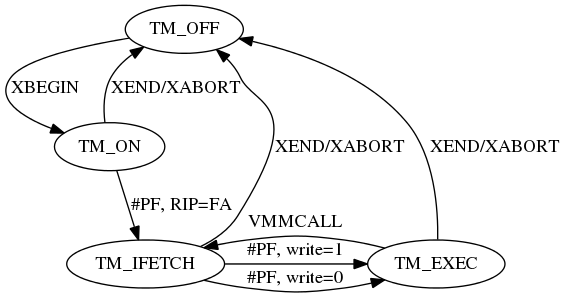
\includegraphics[height=1.75in]{figs/fsm.png}
\caption{The state machine which controls how our implementation records 
transactions. \#PF indicates that a page fault has occurred, FA is the faulting
address, and write indicates the error code.}
\label{flowchart}
\end{figure}
\subsubsection{Beginning a Transaction}

The transaction begins when the VM enounters an XBEGIN instruction. Since the 
VM is running on hardware which does not yet support this instruction, this
causes the VM to exit. On an AMD machine, the SVM handler then indicates that
the undefined exception was indeed the cause for the exit. An undefined 
exception handler is then called, which performs a limited decoding to see
if the exit was caused by one of the three Haswell transactional memory
instructions.    

If the instruction is an XBEGIN, the VMM begins the process of launching the
transaction. First, the argument to XBEGIN is stored, as this indicates the 
location of the failsafe code. A vmmcall is then registered with the VMM
(we further describe this later). Next the various read and write set data
structures are initialised, the transaction state is set to ``IFETCH'', and the
RIP is advanced to the next instruction.

Next, we invalidate the current shadow page table. This will cause the VM to 
exit to Palacios in the event of any memory access, allowing us to record it.
Since we are only eliminating the shadow page table, we are not actually
tampering with the state of the guest, which allows this manipulation to go
undetected by the guest.

\subsubsection{Handling an Ifetch}

Since we have eliminated the shadow page tables, as soon as the VM resumes
executing, a pagefault is caused when attempting to read the instruction.
Since the transaction mode has been set to ON, we are able to catch this
pagefault, and in particular know both the faulting address and the associated
error code. We confirm that this fault is caused by an ifetch through both
the error code and by explicitly checking that the RIP and faulting address
match. We advance the transaction state to ``EXEC'', as we are now executing
a transaction. 
  
In addition, we decode the current instruction in order to determine the length
of its operands. We then replace the next $10$ bytes of instructions with
a VMMCALL. This will allow us to exit back into the VM after the current
instruction has run and perform any updates are necessary. This is particularly
important in the event that an instruction has no memory accesses, so that we
can be sure we are handling each instruction individually. After we do so, 
we return control to the VM.

\subsubsection{Handling a Memory Access}

If we observe a page fault caused in user space while our machine is in the
EXEC state, we know that this is a memory access in our transaction. In the 
event that the error indicates the fault was caused by a read, we first check
our write-set, to see if the address has previously been changed by our 
transaction. If not, we add the page to the read set, then allow the PTE
handler to create the entry normally. However, prior to returning to the VM,
we mark the page as read only, so that attempting to write to it will cause
an additional fault.

If, on the other hand, the address was in our write set, we feed the PTE
handler a special staging page where we store writes. The read then continues
on, using and memory updates performed earlier in the transaction.

If the initial page fault is caused by a write (and in particular, possibly 
caused by an attempt to write on a page that is marked read only), we 
add the page to our write set. We then pass a special staging page to the PTE
handler so that the write is performed on our staging page. This allows the 
writes to appear serially to the processor running the transaction, but be
invisible to all other processors.

Notably, commands which perform a write and a read on the same memory location
will leave the read undetected, as it will not cause a page fault. However,
this will not cause any problems, as a write is strictly worse than a read. In
other words, any situation that would cause an abort with an address in the 
read set will also cause an abort for an address in the write set.

\subsubsection{Finishing an Instruction}

After the memory operations of a given instruction have completed, the 
processor will encounter the VMMCall injected during the ifetch. This will
call the registered handler. This handler will first restore the code that
was overwritten in order to inject the VMMCall. It will then return the state
of the transaction to ``IFETCH''. Finally, the shadow page table is again 
invalidated, to guarantee that the next ifetch, and following memory access 
will cause page faults.  

\subsubsection{Committing An Instruction}

If an XEND instruction is enountered, the ifetch step happens exactly as above.
However, when the VM attempts to execute the instruction, it will exit the VM
and run the undefined exception handler, as with the XBEGIN above. When an XEND
is seen, transaction mode is switched to OFF, the memory in the staging page is
copied to main memory, and control is returned to the VM.

The next instruction will be the injected VMMCall, which will then restore the
replaced code, unregister the hypercall, and return control to the VM without
invalidating the page tables.

\subsubsection{Aborting a Transaction}

As in the hardware implementation, there are numerous reasons why a transaction
may need to be aborted. In addition to the preservation of the serial execution
and atomic commit properties, anything which causes a context switch or general
change to control flow should cause an abort. Additionally the transaction may
abort itself, by calling XABORT. In all of these situations, the state is 
simply switched to ``ABORT''. When the VMMCall runs, it will see that the 
transaction is slated for abortion, clean up the code injection from the ifetch,
and call an abort handler. This handler reasonably disposes of the transaction
data structures and sets the RIP of the VM to the failsafe code, thereby
discarding any changes that the transaction made. 

\subsubsection{External Aborts}

TODO: This I guess.

It is also possible that other threads of execution will trigger an abort by
interacting with the read write sets of the transacting processor. Therefore,
while a transaction is running in one processor, all other cores have their
transaction mode set to OTHER. While this is on, the reads and writes of these
processors are stored using the same techniques as for the transacting
processor, except that all reads and writes are done to main memory instead of
a staging page. If an intersection is ever detected between the transactions
write set and the read and write sets of other cores, or the read set of the
transaction and others write sets, the transaction is aborted, using the same
strategy used for other aborts.  


\section{Design Challenges}

While in the process of designing and implementing this feature in Palacios, we
encountered a number of challenges which ultimately shaped how our implementation
works. The vast majority of the difficulty arises from the need to return
control to Palacios every time a memory operation occurs. Since these normally
occur extremely often with no interference, there is no existing mechanism to 
cause such an action. In order to do so, we chose to make use of shadow paging.
By inducing page faults (namely by blindly invalidating the entire table as
described above), we are able to return control to Palacios nearly every time
an operation occurs.

However, additional mechanisms were still necessary: after an instruction has
completed, we need to again invalidate the shadow tables in order to guarantee 
the next instruction will cause faults. In order to do this, we make use of a 
VMMCall, which we insert after every instruction, as described above. In order
to have the hypercall run the correct handler, the correct code must be moved
into RAX prior to the execution of the call. This adds the further complication
that the value of RAX must also be copied into the guest core data structure,
and restored after the VMMCall has executed, in order to guarantee that the 
transaction code executes correctly.  

In the majority of our tests, we made use of the addq instruction, as the 
decoder is able to properly determine its length and it provides us with the
potential to create a variety of operations. One interesting note, is that when
adding an immediate to a memory address, no detectable read is performed on
the destination address: the first page fault seen after the ifetch is a write.
Therefore, when a transaction is running, and the write is to be done on the
staging page instead of main memory, the instruction will write an incorrect
value on the staging page. For example, adding the immediate $1$ to an address
which contains a $4$ will end up writing $1$ ($0+1$) to a previously blank
staging page. Therefore, when adding a write to the staging page for the first
time, the value in main memory must first be copied to the staging page. While
the solution to this problem was not particularly complex, it stands as an 
example of the complexity that occurs when trying to capture all memory 
activity.
 
- Interrupts

\section{Test Code}

In order to test our implementation, we developed a small set of test code that
performs a small number of memory operations in a way that we can easily check
the correctness of the result when commit or aborting transactions. 
In the simple examples that follow, we use the addq instruction, as it
offers flexibility in the type of operations involving memory we must test.

In general, our code is of the form:
\begin{verbatim}
int main(){
    long x = 1;
    long y = 2;
    printf("%ld\n",x);  
    asm(...)
    printf("%ld\n",x);  
    return 0;
}
\end{verbatim} 

Where the ``asm(...)'' includes our transaction, which should either commit or
abort the result, depending on the test. In the assembly code excerpts below,
we modify $x$, and in some cases, $y$, within a transaction.  For all of these
examples, \%RDX contains the memory address of the variable $x$, while \%RBX
contains the value of $y$.

Our first test file simply adds an immediate value to the contents of a memory
address stored in \%RDX.

\begin{verbatim}
xbeginq 40050e <fail>
addq   $0x1,(%rdx)
xend   
jmp    40050f <success>
\end{verbatim}

In this example, we originally expected the addq instruction to see a page
fault caused by an attempt to read the memory address in \%RDX, however, for
this instruction, the page fault was caused by an attempt to write to the
memory address in \%RDX (which points to our $x$ variable). Originally, when we
mapped this memory address to our staging page, it would perform the read from
the address in the staging page.  In other words, the read and write occurred
simultaneously.  In order to address this issue, even when we page fault due to
a write, we first read the current contents of memory and save it to our
staging page. Then the write is actually performed to the staging page, using
the initial value we copied.  After reaching the xend instruction,  Then it
copies the result back to the main memory upon the successful completion of the
transaction, causing the final printf to output a $2$.

Next, we test the adding of a memory address to a register:

\begin{verbatim}
xbeginq 400518 <fail>
add    (%rdx),%rax
xend   
jmp    400519 <success>
\end{verbatim}

In this case, we expect to single page fault caused by the read to the address
in \%RDX register. Again, this happens as expected, and the address is logged
in the appropriate read set. When \%RAX is initialized to 0, the process 
successfully prints $1$ upon completion.


In our next example, we look at a slightly more complicated case where we first
modify a value in memory, and then use the written value in a subsequent
instruction. This checks to ensure that we are properly using values from the
staging page. 

\begin{verbatim}
xbeginq 40051e <fail>
addq   $0x1,(%rdx)
add    (%rdx),%rbx
xend   
jmp    40051f <success>
\end{verbatim}

As with the first example, this first adds one to $x$ (in memory). Next it
reads the value from memory, and adds it to \%RBX. Here, \%RBX contains the
value of $y$.  Upon successful completion of the program it prints $4$ ({1 + 1
+ 2}).


Our last test program directly tests our ability to rollback a commit when we
reach an xabort.

\begin{verbatim}
xbeginq 40051e <fail>
addq   $0x1,(%rdx)
xabort $5
\end{verbatim}

Here, we once again modify the value stored in $x$. However, this time, we hit
an xabort before reaching an xend statement.  As soon as we hit the invalid
instruction for the xabort, we call our abort handler to free our data
structures and roll back our changes. As a result, the change to $x$ appears as
though it never occurred. We then modify \%RIP according to the argument to the
xbegin statement. Although we only tested the aborts directly with xabort, the
same abort handler could be called from whenever an event occurs that
invalidates the transaction, such as a conflicting write from another core.

\subsection{Current Assumptions}

The current implementation in palacios is subject to a number of assumptions
that are currently the result of time limitations, and not intended to be a
part of the final transaction model.

First, due to simplicity, the undefined exception hander only runs on AMD 
processors which provide the SVM extension. Additionally, the injected 
hypercalls are currently using the AMD model. Both of these are likely to be
trivial to implement via their Intel counterparts.  

In order to perform the hypercall code injection, the decoder is used to 
determine the length of the current instruction, so that the injected code
can be placed without damaging neceassary operands. However, the built in
decoder currently only works with a limited set of instructions, preventing
arbitrary instructions from being run in a transaction, limiting them to a 
small set of test instructions. While this issue can likely be solved by 
switching to the QUIX86 decoder \cite{quix86site}, as it can handle a much larger
instruction set, bugs in Palacios prevented us from doing so at this time.

The current implementation also assumes that the set of instructions in a 
transaction occur on the same page, and do not run within $10$ bytes of the
end of the page. While this should be fixable by checking the alignment of
the instruction address, we have left this assumption in the interest of 
time. 

The current staging page used to store the writes done by a transaction also
makes two assumptions. First, we require that all memory written by a 
transaction fit on a single page. While this is not unreasonable, given that
transactions are intended, in general, to be smaller, it does create an
artificial limitation. Second, since the handler which deals with the case
of a transaction write simply passes the usual PTE handler the same staging
page no matter what, it assumes that the offset will not conflict with any
previous or future writes. We see that this could happen if two writes which
normally happen on separate pages, but the same offset, are performed in the
same transaction. Again, while this scenario is unlikely for small transactions
we are creating a restriction.
 
During testing, we observed that after every reentry to the VM, a number
of interrupts occur, and control jumps to the kernel. While we have not yet
determined the cause of these interrupts, we suspect they are the result of 
a timer, or other piece of hardware. Since these may interfere with our 
transaction, we should abort when this occurs. However, since our test 
transactions are simple, we assume that they will not interfere with a 
transaction and simply ignore the interrupts. In particular, this means that
we ignore a wave of page faults on kernel address upon each return to the
VM. Since the error code of the fault indicates the faults were raised by
the kernel, we can easily filter them out.   

The transaction mode indicator currently assumes that only a single
transaction can run at a time. This means that if one process is in transaction
mode, a second core encountering an XBEGIN instruction will cause problems.
This could be worked around without too much difficulty by separating the
indicators, allowing a core to be in both transaction mode (ie performing
a local transaction), and recording its writes to be validated against
another transaction.

Our current implementation also assumes that it is the only core running, and
ignores the potential of aborts cause by threads of execution on other cores.
While this assumption must be removed in order for transactional memory to
truly be effective, this has allowed us to implement much of the basic tools
and structure necessary for transactional memory.
 

\section{Future Work}

Future directions for this work are clear: extend the current rudimentary 
implementation until it is fully compatible with the Intel specifications. In
particular, this means eliminating many of the limiting assumptions that were
made in the presented design.

First, the limitation that instructions must fit on a page could be solved by
checking the address of the instruction prior to the code injection. If the 
instruction is too near the edge of a page, appropriate steps could be taken
to properly inject and restore the code. While this is again not overly 
difficult, it does add significant complexity to the instruction injection
mechanism.

The assumptions related to the staging page (that all writes fit on a page
and that none of the writes have overlapping offsets), could be eliminated
by no longer using the staging page as a master copy of memory for a 
transaction, but instead using it as a place for scratch work. When a 
write occurs, we pass the PTE handler the staging page, as before, but when we 
next exit via the hypercall, we copy the result of the write to the write set
data structure. When performing a read on an address in the write set,
we first copy the data to the staging page, ensuring that the read sees the
newest possible version.

There are more complex behaviors described, which are not yet
implemented, but so not depend on any general structural changes. For example,
the Intel specification allows for nested transactions in certain situations.
Implementing this would likely only require minor modifications to the state
machine. 

Finally, there is the issue of performance. While our implementation is able 
to capture and record all operations that it needs to track, it does so at the
cost of up to $4$ exits per instruction, which would result in a tremendous
slowdown. It is likely that the necessary information could be retrieved at a 
less granular scale and reduce the number of exits to Palacios.

One proposed solution is to emulate all instructions within a transaction,
and therefore handling the entire transaction in the host. While this would
eliminate the number of exits and entries, implementing an emulator and managing
the transaction are non-trivial endeavors. 
  
\section{Conclusions}

We have implemented the preliminary components of support for the Intel model
of transactional memory in the Palacios virtual machine manager. Despite a 
number of complex technical challenges, we have been able to create
transactions which are able to log their memory activity, and either commit
the data to main memory, or abort it in the case of interference. While the
current implementation is subject to a number of restrictions, we have 
completed a number of the core components, which should greatly simplify 
the remainder of the task.

More generally, we have demonstrated that Palacios, and virtual machines in
general, stand to provide a powerful platform for the design and testing of
future hardware mechanisms. Using the power and control of Palacios, numerous
other paradigms could be tested, without waiting for expensive, and possibly
incomplete, implementations from hardware manufacturers. Furthermore, it could
greatly simplify simulations for such hardware testing tools. 

\section{Author Bios}

Zachary Bischof is a third-year PhD student working with Prof. Fabi\'{a}n
Bustamante in the AquaLab research group. His research interests include
networking and distributed systems, in particular, evaluating their performance
and impact on the network.

Marcel Flores is a first year PhD student of Prof. Aleksander Kuzmanovic in the
Networking group. His research interests include studying the preservation of
user privacy and how to use high level web information to inform network
systems.

Maciej Swiech is a first year PhD student of Peter Dinda in the Empathic
Systems Project. His research interests include real-world implementations of
empathic systems, power optimization in mobile platforms, and low-level systems
work.

\bibliography{transmem}

\end{document}
